\documentclass[letterpaper]{article}
\usepackage{amsmath, geometry, graphicx, tikz}
\usetikzlibrary{arrows.meta}
\bibliographystyle{plain}

\title{Regulators and Psychiatric Associates of Genomic Imprinting in the Human Brain}
\author{Attila Guly\'{a}s-Kov\'{a}cs\(^\ast\), Ifat Keydar\(^\ast\),
...,
%\\
%Eva Xia, Menachem Fromer, Doug Ruderfer,\\
%Ravi Sachinanandam,
Andrew Chess}
\date{Mount Sinai School of Medicine}

\begin{document}

\maketitle

\section{Supplementary Figures}

\setcounter{figure}{0}
\makeatletter 
\renewcommand{\thefigure}{S\@arabic\c@figure}
\makeatother

\begin{figure}
\begin{center}
\includegraphics[scale=0.6]{figures/2016-08-08-imprinted-gene-clusters/score-genomic-location-1.png}
\end{center}
\caption{
Clustering of top-scoring genes in the context of human DLPFC around genomic locations that
had been previously described as imprinted gene clusters in other contexts.
}
\label{fig:clusters}
\end{figure}

\begin{figure}
\begin{center}
\includegraphics[scale=0.6]{figures/2016-08-01-ifats-filters/known-genes-1.pdf}
\caption{Known imprinted genes ranked by the gene score (dark blue bars).
``Known imprinted'' refers to prior studies on imprinting in the context of
any tissue and developmental stage.  The length of the
black bars indicates the fraction of individuals passing the test of nearly
unbiased expression.}
\label{fig:known-genes}
\end{center}
\end{figure}

\begin{figure}
\begin{center}
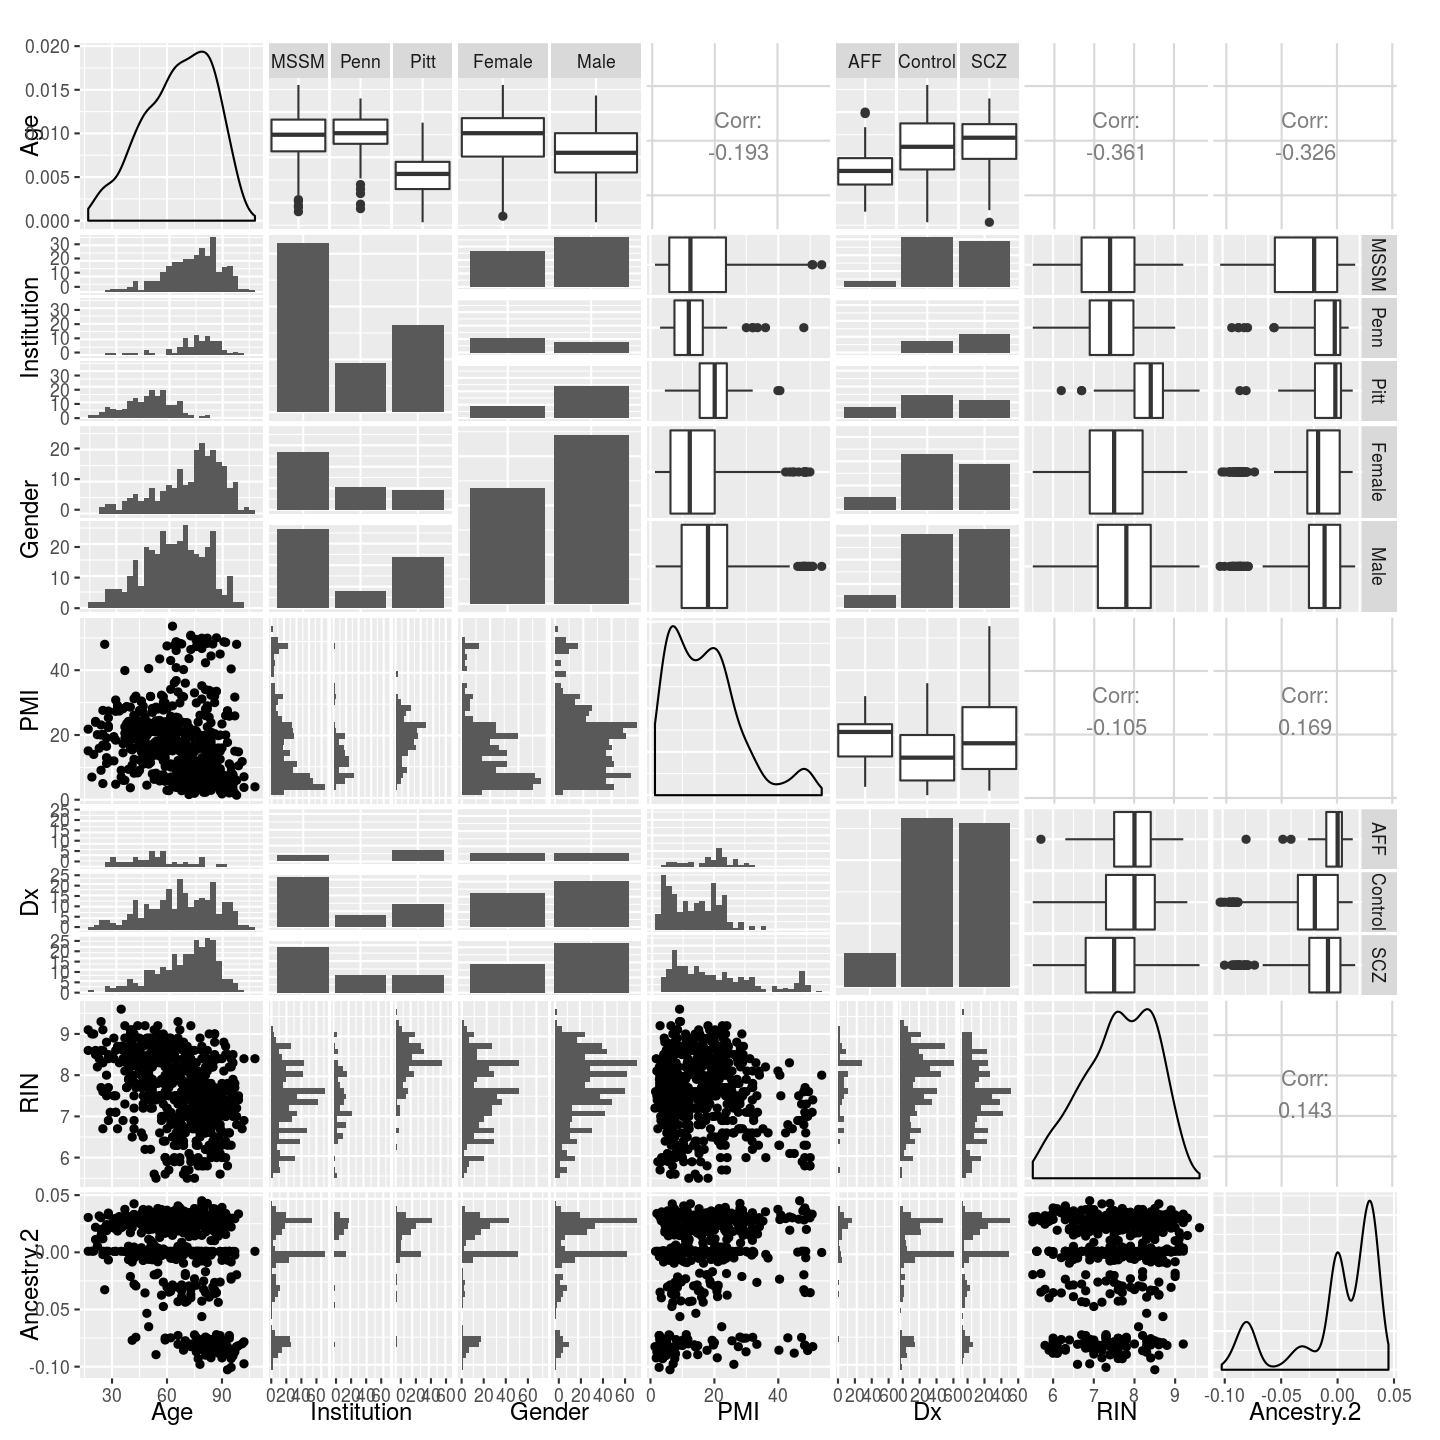
\includegraphics[scale=0.6]{figures/2016-06-26-trellis-display-of-data/evar-scatterplot-matrix-2.png}
\end{center}
\caption{
Pairwise dependencies among predictors.
}
\label{fig:predictor-associations}
\end{figure}

\begin{figure}
\begin{center}
\includegraphics[scale=0.6]{figures/2016-06-26-trellis-display-of-data/S-age-gender-1.png}
\caption{
Variation of the read count ratio \(S_{ig}\) with age and gender across hundreds of individuals
\(i\) (dots) and 30 genes \(g\) that have been considered as imprinted in the DLPFC
brain area in this study.
}
\label{fig:S-age-gender}
\end{center}
\end{figure}

\begin{figure}
\begin{center}
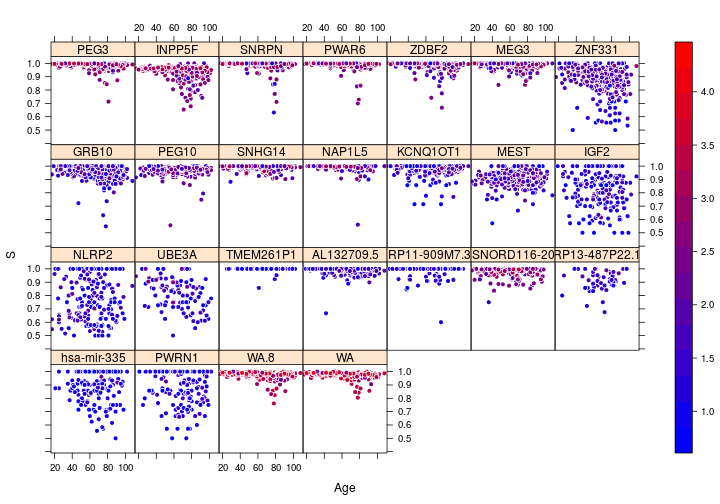
\includegraphics[scale=0.6]{figures/2016-06-26-trellis-display-of-data/S-age-tot-read-count-1.png}
\end{center}
\caption{Variation of total RNA-seq read count across genes and individuals.}
\label{fig:weight-of-evidence}
\end{figure}

\begin{figure}
\begin{center}
\includegraphics[scale=0.6]{figures/2016-09-23-model-checking/qqnorm-wnlm-Q-1.pdf}
\end{center}
\caption{
Checking the fit of wnlm.Q model: analysis of the normality of residuals.
}
\label{fig:qqnorm-wnlm.Q}
\end{figure}

\begin{figure}
\begin{center}
\includegraphics[scale=0.6]{figures/2016-09-23-model-checking/qqnorm-logi-S-1.pdf}
\end{center}
\caption{
Checking the fit of logi.S model: analysis of the normality of standardized deviance residuals.
}
\label{fig:qqnorm-logi.S}
\end{figure}

\begin{figure}
\begin{center}
\includegraphics[scale=0.6]{figures/2016-09-23-model-checking/homoscedas-wnlm-Q-1.pdf}
\end{center}
\caption{
Checking the fit of wnlm.Q model: analysis of homoscedasticity.
}
\label{fig:homoscedas-wnlm.Q}
\end{figure}

\begin{figure}
\begin{center}
\includegraphics[scale=0.6]{figures/2016-09-23-model-checking/homoscedas-logi-S-1.pdf}
\end{center}
\caption{
Checking the fit of logi.S model: analysis of homoscedasticity.
}
\label{fig:homoscedas-logi.S}
\end{figure}

\begin{figure}
\begin{center}
\includegraphics[scale=0.6]{figures/2016-09-23-model-checking/influence-wnlm-Q-1.pdf}
\end{center}
\caption{
Checking the fit of wnlm.Q model: analysis of the impact of outliers.
}
\label{fig:influence-wnlm.Q}
\end{figure}

\begin{figure}
\begin{center}
\includegraphics[scale=0.6]{figures/2016-09-23-model-checking/influence-logi-S-1.pdf}
\end{center}
\caption{
Checking the fit of logi.S model: analysis of the impact of outliers.
}
\label{fig:influence-logi.S}
\end{figure}

\begin{figure}
\begin{center}
\includegraphics[scale=0.6]{figures/2016-10-03-permutation-test/p-val-tdist-vs-perm-filt-iso-1.pdf}
\end{center}
\caption{Agreement between a parametric (t-distribution) and non-parametric
(permutations) method of estimating p-values.}
\label{fig:pval-tdist-vs-perm}
\end{figure}

\begin{figure}
\begin{center}
\includegraphics[scale=0.6]{figures/2016-10-03-permutation-test/p-values-1.pdf}
\end{center}
\caption{
Significance of association between biological predictors and imprinted genes
in the DLPFC calculated under wnlm.Q and logi.S.  Under logi.S, only those
genes are shown for which the model fit was acceptable.
}
\label{fig:pval}
\end{figure}

\begin{figure}
\begin{center}
\includegraphics[scale=0.6]{figures/2016-08-08-imprinted-gene-clusters/segplot-logi-S-99conf-1.pdf}
\end{center}
\caption{
Estimate \(\hat{\beta}_{jg}\) and 99\% confidence interval of each regression coefficient
\(\beta_{jg}\) under the logi.S model, where \(j\) is a predictor/term and
\(g\) is a gene.  \(\hat{\beta}_{jg}\) and the confidence interval are shown only for those
genes are shown for which the model fit was acceptable.
}
\label{fig:biol-effects-logi.S}
\end{figure}

\begin{figure}
\begin{center}
\includegraphics[scale=0.6]{figures/2016-08-21-likelihood-surface/explain-rll-wireframe-1.png}
\includegraphics[scale=0.6]{figures/2016-08-21-likelihood-surface/explain-rll-levelplot-B-1.png}
\end{center}
\caption{
\emph{Top} and \emph{bottom}: two representations of the relative log
likelihood on a 2 dimensional section of the \(p>20\) dimensional parameter
space given the wnlm.Q model and data for the gene \(g=\mathrm{PEG3}\).  The
section was taken by fixing all but two parameters at their estimates:
\(\beta_{jg} = \hat{\beta}_{jg}\).  A rectangular subspace for these two
parameters, \(\beta_{\mathrm{Age},g}\) and  \(\beta_{\mathrm{Ancestry.2},g}\),
was chosen around the maximum likelihood estimate \(\hat{\beta} =
(\hat{\beta}_{\mathrm{Age},g}, \hat{\beta}_{\mathrm{Ancestry.2},g})\).  The
nearly parabolic shape of the log-likelihood function suggests that the
regularity conditions for likelihood-based parametric inference are fulfilled.
}
\label{fig:ll-surf-explain}
\end{figure}

\begin{figure}
\begin{center}
\includegraphics[scale=0.6]{figures/2016-06-22-extending-anova/logi-S-wnlm-Q-compare-1.pdf}
\end{center}
\caption{
Agreement of the wnlm.Q and logi.S models in terms of estimated regression
coefficients.
}
\label{fig:logi.S-wnlm.Q-compare}
\end{figure}

\begin{figure}
\begin{center}
\includegraphics{figures/by-me/monoall-dependencies-2/obs-simple-general/obs-simple-general}
\hspace{\fill}
\includegraphics{figures/by-me/monoall-dependencies-2/obs-simple-general-gene-aspec/obs-simple-general-gene-aspec}
\hspace{\fill}
\includegraphics{figures/by-me/monoall-dependencies-2/obs-bayesian/obs-bayesian}
\end{center}
\caption{ General dependency structure of three regression model frameworks.
In all of threse model frameworks the regression coefficients
\(\beta_{1g},...,\beta_{3g}\) mediate, for a given gene \(g\), probabilistic
dependencies (arrows) between the response variable \(Y_g\) (read count ratio
for \(g\)) and the corresponding predictors \(X_1,...,X_3\).  For simplicity
but without loss of generality only 3 predictors are depicted.  The model
frameworks differ in how \(\beta_{jg_1},\beta_{jg_2},...\) relate to each
other for a given predictor (or a given \(j\)).  \emph{Left:} there is no
connection among \(\beta_{jg_1},\beta_{jg_2},...\) which means that the way
\(Y_{g}\), the read count ratio for gene \(g\) depends on predictor \(X_j\) is
completely separate from how the read count ratio for any other gene \(g'\)
(i.e.~\(Y_{g'}\)) depends on it.  Consequently no information may be shared
among gene-specific models.  \emph{Middle:} In this case
\(\beta_{jg_1}=\beta_{jg_2}=...\equiv\beta_j\) so that all genes are identical
with respect to how their read count ratio depends the predictors.  Thus genes
share all information in the data in the sense that the model forces them to
be identical.  \emph{Right:} Hierarchical Bayesian model where genes show both
variation as well as invariance with regards to depenencies.  The variation is
described by the dependence of \(\beta_j\) on the hyperparameter \(\gamma_j\),
whereas the invariance by the dependence of \(\gamma_j\) on \emph{its}
hyperparameter \(\xi_j\).  Only this model framework allows information
sharing among genes in a flexible way.  }
\label{fig:glm-vs-hierarch}
\end{figure}

\begin{figure}
\begin{center}
\includegraphics[scale=0.6]{figures/2016-06-22-extending-anova/reg-coef-wnlm-Q-1.pdf}
\end{center}
\caption{
Estimates \(\hat{\beta}_{jg}\) and confidence intervals for regression
coefficients under the wnlm.Q model concerning for all predictors.
}
\label{fig:all-effects-wnlm.Q}
\end{figure}

\begin{figure}
\begin{center}
\includegraphics[scale=0.6]{figures/2016-06-22-extending-anova/reg-coef-logi-S-filt-1.pdf}
\end{center}
\caption{
Estimates \(\hat{\beta}_{jg}\) and confidence intervals for regression
coefficients under the logi.S model concerning for all predictors.  Gaps
for certain genes indicate unacceptable fit.
}
\label{fig:all-effects-logi.S}
\end{figure}

\begin{figure}
\begin{center}
\includegraphics[scale=0.6]{figures/2016-08-21-likelihood-surface/ll-surf-coefs-wnlm-Q-1.png}
\end{center}
\caption{
Analysis of orthogonality of regression coefficients.  Relative log-likelihood
surfaces for the gene PEG3 on various rectangles corresponding to 2D sections
through the \(p>20\) dimentional parameter space.  The set of points in a
rectangle where log-likelihood takes the same value are quasi-ellipses, whose
major and minor axes and their tiltedness express association between
coefficients.  For instance, \(\beta_\mathrm{Age}\) is not assiciated with
(orthogonal to) \(\beta_\mathrm{Ancestry.2}\) but is strongly associated with
\(\beta_\mathrm{RIN}\).  Such association hinders statistical inference due to
the following circularity: If we knew the precise value of
\(\beta_\mathrm{RIN}\) we could estimate the true value of
\(\beta_\mathrm{Age}\) with higher precision and confidence but the precise
value of \(\beta_\mathrm{RIN}\) could only be obtained with high confidence if
we precisely knew \(\beta_\mathrm{Age}\).
}
\label{fig:ll-non-orthogonality}
\end{figure}

\begin{figure}
\begin{center}
\includegraphics[scale=0.6]{figures/2016-07-08-conditional-inference/beta-age-cond-wnlm-Q-2-1.pdf}
\end{center}
\caption{
Analysis of interactions among predictors under the wnlm.Q model.  Contextual depenendence of the
read count ratio on age, where the context is given by some specific level of
Institution (MSSM, Penn, Pitt) or Gender (Female, Male).
}
\label{fig:interaction-wnlm.Q}
\end{figure}

\begin{figure}
\begin{center}
\includegraphics[scale=0.6]{figures/2016-07-08-conditional-inference/beta-age-cond-logi-S-2-skip-1.pdf}
\end{center}
\caption{
Analysis of interactions among predictors under the logi.S model.  The missing
panels correspond to genes for which logi.S did not provide acceptable fit.
}
\label{fig:interaction-logi.S}
\end{figure}

\begin{figure}
\begin{center}
\includegraphics[scale=0.6]{figures/2016-06-22-extending-anova/anova-effects-fw-rv-wnlm-Q-1.pdf}
\end{center}
\caption{
\emph{Left:} analysis of variance (ANOVA) is undermined by the non-orthogonality of
predictors because the reduction in deviance (i.e.~in residual sum of squares)
for a term (predictor) depends on the sequence in which terms are added to the
model.  \emph{Right:} the same concept is demonstrated using QR decomposition.
}
\label{fig:anova}
\end{figure}

\begin{figure}
\begin{center}
\includegraphics[scale=0.6]{figures/2016-10-20-differential-expression-scz/venn-triple-1.pdf}
\end{center}
\caption{
Association of genes' expression to schizophrenia (SCZ) assayed by two RNA-seq
based approaches: total read count (overall expression, Nat Neurosci.~2016
Nov;19(11):1442-1453.)~and read count ratio
(allelic bias, present work).  When these approaches are compared for only
those genes that we find imprinted in the DLPFC in this study, 1 gene is found
associated to schizophrenia by both approaches, 1 by only overall expression,
and 3 by only allelic bias.
}
\label{fig:diff-exp-scz}
\end{figure}

%\begin{figure}
%\includegraphics[width=0.6\textwidth]{figures/2016-10-11-comparison-to-mouse-cerebellum/posterior-pp-vs-pval-wnlm-Q-1.pdf}
%\caption{Comparison of the effects of age and gender between the present work and a
%previous study~\cite{Perez2015} in the mouse cerebellum. }
%\label{fig:mouse-cerebellum}
%\end{figure}

% Supplementary tables

\setcounter{table}{0}
\makeatletter 
\renewcommand{\thetable}{S\@arabic\c@table}
\makeatother

\end{document}
